\section{Vstupní data a předzpracování}
\label{sec-modelAnalysis}
Aplikace načítá celou řadu dat, se kterými dále pracuje. V první řadě je nutné načíst popis stromu, dále pak textury použité pro jeho zobrazení. Načtená data je v řadě případů nutno předzpracovat, aby je bylo možné využít. Právě popisem vstupních dat a jejich předzpracováním se bude zabývat následující text.

%%%%%%%%%%%%%%%%%%%%%%%%%%%%%%%%%%%%%%%%%%%
\subsection{Formát OBJT}
Jelikož běžné modely stromů neobsahují implicitně informace o topologii stromu, která je nezbytná pro provedení animace, byl navržen formát vstupního souboru OBJT, který zahrnuje právě tyto informace. Soubor formátu OBJT je vstupním souborem popisujícím model stromu. OBJT je textový formát obsahující 4 druhy záznamů (oddělených standardním oddělovačem řádků):
\begin{itemize}
\item pojmenování stromu na začátku souboru entitou \lineCode{name = "\%sting\%"}
\item entita popisující větev \begin{verbatimtab}
B  %int% { 			// identifikátor větve
  l   	%int%			// úroveň v hierarchii
  d 	%float%			// délka větve
  z  	%float%	%float%	%float%	// pozice začátku větve
  k 	%float%	%float%	%float%	// pozice konce větve
  r  	%float%	%float%	%float%	// bázový vektor r
  s  	%float%	%float%	%float%	// bázový vektor s
  t  	%float%	%float%	%float%	// bázový vektor t (podélný)
  p  	%int%			// identifikátor rodičovské větve
  x  	%float%	// v kolikátině rodičovské větve se větev odpojuje
}
\end{verbatimtab}
\item entita popisující list  \begin{verbatimtab}
L  %int% { 			// identifikátor listu
  r  	%float%	%float%	%float%	// bázový vektor r
  s  	%float%	%float%	%float%	// bázový vektor s
  t  	%float%	%float%	%float%	// bázový vektor t (podélný)
  p  	%int%			// identifikátor rodičovské větve
  x  	%float%	// v kolikátině rodičovské větve se list odpojuje
}
\end{verbatimtab}
\item řádkový komentář začínající \lineCode{// \%string\%}
\end{itemize}

Ve výše uvedeném popisu formátu jsou použity zástupné řetězce za celá čísla (\lineCode{\%int\%}), za desetinná čísla (\lineCode{\%float\%}) a za znakové řetězce bez oddělovače konce řádků (\lineCode{\%string\%}). Všechny souřadnice se předpokládají v souřadném systému celého stromu (též \emph{object space}).

Data ze zdrojového OBJT jsou načtena, větve jsou vytvořeny jako kužely a listy jako ploché čtverce (quads). Vrcholy a jejich atributy jsou následně uloženy do VBO. Těmito daty jsou:
\begin{itemize}
\item pozice v souřadném systému větve
\item normála a tangenta v souřadném systému rodičovské větve
\item texturovací souřadnice
\item vektor hodnot x (viz obr.~\ref{fig:hierarchyCoords})
\item souřadnice do datové textury pro příslušnou větev (její obsah bude popsán dále)
\end{itemize}

%%%%%%%%%%%%%%%%%%%%%%%%%%%%%%%%%%%%%%%%%%%
\subsection{Textury}
\label{sec:Textury}
Ačkoliv je v celé aplikaci použito velké množství textur (pro skybox, krajina, atd.), zde budou zmíněny pouze ty nejdůležitější, které se vážou přímo k tématu zobrazování stromů.

Pro zobrazení 3D modelu stromu je použito několik textur, které jsou načítány při spuštení aplikace. Kromě textur použitých pro zobrazení listů (viz obr.~\ref{fig:leafResources}) je pro obarvení kmene a větví načtena textura jejich struktury (viz obr.~\ref{fig:branchResources}).
\begin{figure}[!hbt]
\begin{center}
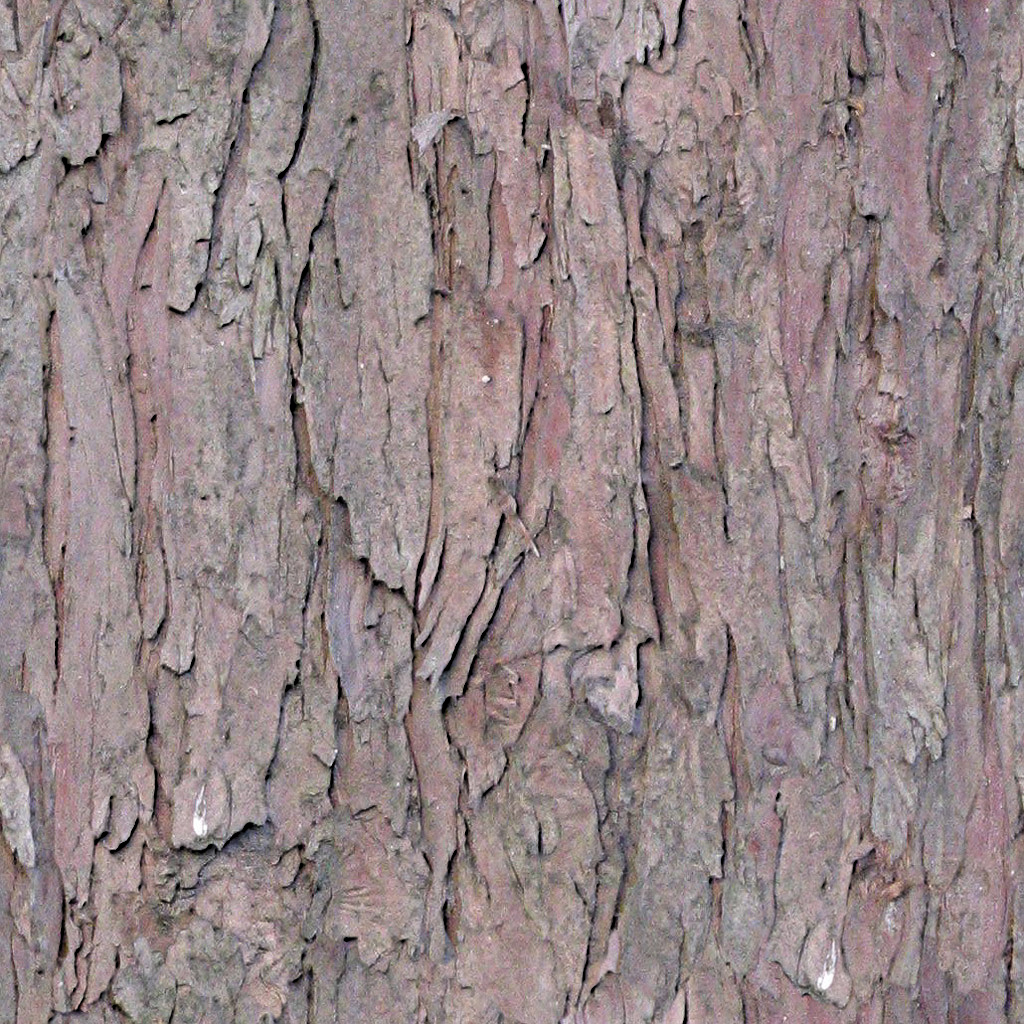
\includegraphics[width=0.35\textwidth]{./figures/bark2_decal.png}
\end{center}
\caption[Zdrojová textura barvy kmene a větví]%
{Zdrojová textura barvy kmene a větví. \label{fig:branchResources}
}
\end{figure}

Dále jsou načteny šumové textury řídící animaci (obr.~\ref{fig:noiseResources})
\begin{figure}[!hbt]
\begin{center}
$\begin{array}{cc}
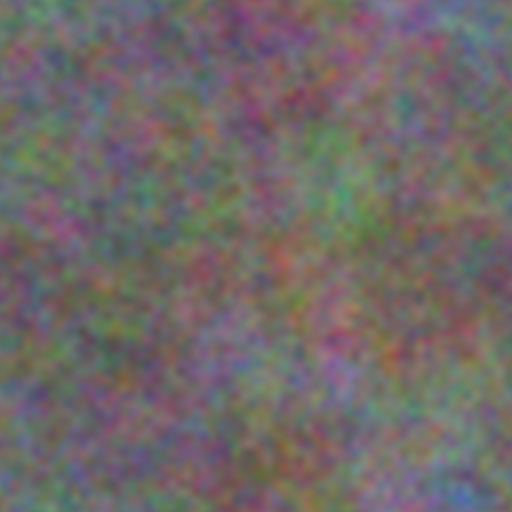
\includegraphics[width=0.4\textwidth]{./figures/branch_noise.png}&
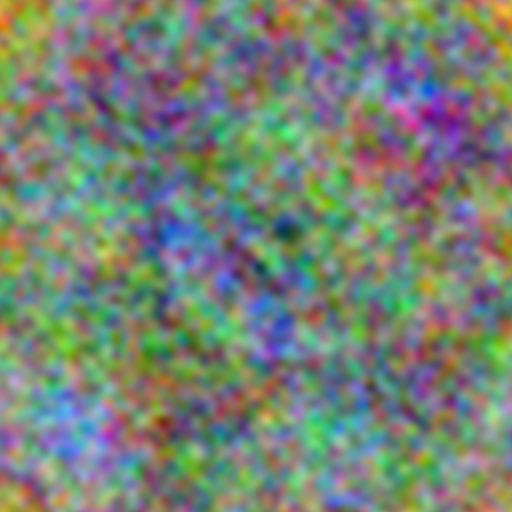
\includegraphics[width=0.4\textwidth]{./figures/leaf_noise.png}\\
(a)&(b)
\end{array}$
\end{center}
\caption[Šumové textury animace větví a listů]%
{Šumové textury animace větví (a) a listů (b) \label{fig:noiseResources}
}
\end{figure}

Přímo zásadní je však textura, v níž jsou uložena data potřebná pro provedení deformace ve vertexovém procesoru. Tuto texturu je nutné pro daná vstupní data popisující strom vytvořit.
Pro její sestavení je třeba převést zejména bázové vektory větve ($\vec{r}$, $\vec{s}$, $\vec{t}$) do souřadného systému rodičovské větve (převedené vektory $\vec{r_b}$, $\vec{s_b}$, $\vec{t_b}$). Zároveň je potřeba pro každou větev vytvořit (pokud možno) unikátní vektor $\vec{mv}$ posunu v šumové textuře. Informace doplňují záznamy o délkách rodičovských větví $l_0-3$. Jelikož je třeba uložit do textury normalizované vektory, je použita textura typu \lineCode{GL\_RGBA32F}. 

Minimální sada dat v datové textuře tedy vypadá následovně:
\begin{table}[!hbt]
\catcode`\-=12
\begin{center}
\begin{tabular}{c | c | c | c | c | c | c | c | c | c | c |} 
 & \multicolumn{10}{c}{obsah textury}\\
i+1 & \multicolumn{10}{c |}{\vdots}\\
\cline{1-11}
\multirow{4}{*}{i} & $\vec{mv_0}.x$ 	& $\vec{mv_2}.x$ 	&  $\vec{s_{b,0}}.x$  & $\vec{s_{b,1}}.x$  & $\vec{s_{b,2}}.x$  & $\vec{s_{b,3}}.x$  & $\vec{r_{b,0}}.x$  & $\vec{r_{b,1}}.x$  & $\vec{r_{b,2}}.x$  & $\vec{r_{b,3}}.x$\\
\cline{2-11}
& $\vec{mv_0}.y$ 		& $\vec{mv_2}.y$ 	&  $\vec{s_{b,0}}.y$  & $\vec{s_{b,1}}.y$  & $\vec{s_{b,2}}.y$  & $\vec{s_{b,3}}.y$  & $\vec{r_{b,0}}.y$  & $\vec{r_{b,1}}.y$  & $\vec{r_{b,2}}.y$  & $\vec{r_{b,3}}.y$\\
\cline{2-11}
& $\vec{mv_1}.x$ 		& $\vec{mv_3}.x$  	&  $\vec{s_{b,0}}.z$  & $\vec{s_{b,1}}.z$  & $\vec{s_{b,2}}.z$  & $\vec{s_{b,3}}.z$  & $\vec{r_{b,0}}.z$  & $\vec{r_{b,1}}.z$  & $\vec{r_{b,2}}.z$  & $\vec{r_{b,3}}.z$\\
\cline{2-11}
& $\vec{mv_1}.y$ 		& $\vec{mv_3}.y$ 	&  $l_0$  &$l_1$  & $l_2$ & $l_3$  &  & & & \\
\hline
i-1 & \multicolumn{10}{c |}{\vdots}\\
\end{tabular}
\label{table:dataTexture}
\caption{Minimální sada dat uložená v datové textuře.}
\end{center}
\end{table}

\begin{figure}[!hbt]
\begin{center}

\includegraphics[width=0.05\textwidth]{./figures/branchDataTextureLOD0.png}
\end{center}
\caption[Ukázka z datové textury pro LOD0]%
{Ukázka z datové textury pro LOD0. Číslo řádku $i$ odpovídá identifikátoru větve.\label{fig:branchDataTextureLOD0}
}
\end{figure}


Zobrazování LOD1 a LOD2 vyžaduje rovněž vytvoření několika speciálních textur. Jejich vytvořením se zabývá další sekce (~\ref{sec:preprocessLOD}).


%%%%%%%%%%%%%%%%%%%%%%%%%%%%%%%%%%%%%%%%%%%
\subsection{Předzpracování pro LOD}
\label{sec:preprocessLOD}
Pro zobrazení a animaci LOD1 a LOD2 je třeba vytvořit během předzpracování sadu textur. Jednak je to množina textur, které jsou nezbytné i pro zobrazení statického stromu, druhak se pak přidávají i textury, jež jsou nezbytné pro provedení animace. Následující popis uvádí postup generování těchto textur pro LOD1. Pro LOD2

Ke zobrazení statického stromu pomocí trsu řezů je třeba vytvořit textury obsahující pohled na strom z daného úhlu v několika vrstvách. Tyto textury lze relativně jednoduše generovat použitím techniky \emph{offscreen-rendering} neboli vykreslování do textur. V OpenGL se toho dosáhne připojením speciálního tzv. \emph{Frame Buffer Object} (FBO) s napojenými texturami. Následující kód ukazuje, jak takovýto FBO vytvořit a použít:
\pagebreak
\begin{alltt}
\textit{// vytvoreni FBO}
GLuint	fboID = 0;
GLenum buffers[3] = \{ GL_COLOR_ATTACHMENT0,
                      GL_COLOR_ATTACHMENT1,
                      GL_COLOR_ATTACHMENT2 \};
glGenFramebuffers(1, &fboID);
glBindFramebuffer(GL_FRAMEBUFFER, fboID);
   glFramebufferTexture2D(GL_FRAMEBUFFER, GL_COLOR_ATTACHMENT0, GL_TEXTURE_2D,
                          colorTextureID, 0);
   glFramebufferTexture2D(GL_FRAMEBUFFER, GL_COLOR_ATTACHMENT1, GL_TEXTURE_2D,
                          normalTextureID, 0);
   glFramebufferTexture2D(GL_FRAMEBUFFER, GL_COLOR_ATTACHMENT2, GL_TEXTURE_2D, 
                          branchTextureID, 0);
   glFramebufferTexture2D(GL_FRAMEBUFFER, GL_DEPTH_ATTACHMENT, GL_TEXTURE_2D, 
                          depthTextureID, 0);
glBindFramebuffer(GL_FRAMEBUFFER, NULL);

\textit{// pouziti FBO}
{\bf setupCamera();}      \textit{// nastaveni kamery podle smeru a hloubky rezu}
glBindFramebuffer(GL_FRAMEBUFFER, fboID);
      glDrawBuffers(3, buffers);			
           {\bf draw();}     \textit{// vykresleni do pripojenych textur}
      glDrawBuffer(GL_BACK);
glBindFramebuffer(GL_FRAMEBUFFER, NULL);
\end{alltt}

Pro generování řezů je kamera nastavena na orthogonální projekci a vykreslení pouze určitého řezu je zajišteno správným nastavením přední a zadní ořezové roviny kamery ($near$, $far$). Jelikož se v této fázi vykresluje celý strom v normované jednotkové velikosti, je určení hodnot $near$ a $far$ triviální pro $i$-tý řez z daného směru : 
\begin{align}
thickness &= \frac {diameter_{tree}}{count_{slice}}\nonumber \\
near_i &= distance_{camera}-(0.5 \cdot diameter_{tree}) + i \cdot thickness \nonumber\\
far_i &= near_i + thickness
\end{align}

Nastavení projekční matice kamery zajišťuje funkce:
\begin{alltt}
glOrtho(float l, float r, float b, float t, float {\bf near}, float{\bf  far});
\end{alltt}

Pro každý řez je vytvořena následující sada textur:
\begin{itemize}
\item barevná textura
\item hloubková textura
\item normálová textura
\item textura větvových bodů
\end{itemize}

Do textur je vykreslen geometrický model v základní pozici (neovlivněný působením větru). Do barevné textury se zapíše nestínovaná barva bez sezónní složky, do textury normál se zapíše pro každý fragment normála (pouze 3 souřadnice) v souřadném systému řezu (budoucí \emph{tangent space}). Čtvrtá složka zaznamenává případně specifické číslo listu. Význam hloubkové mapy je zřejmý. Do textury větvových bodů se zaznamenávají identifikátory rodičovských větví 1. úrovně (napojené přímo na kmen). Následně je na této textuře provedena expanze dat (viz obr.~\ref{fig:dataExpansionExample}).

%%%
% obrazek pred a po expanzi dat
%
\begin{figure}[!hbt]
\begin{center}
$\begin{array}{cc}
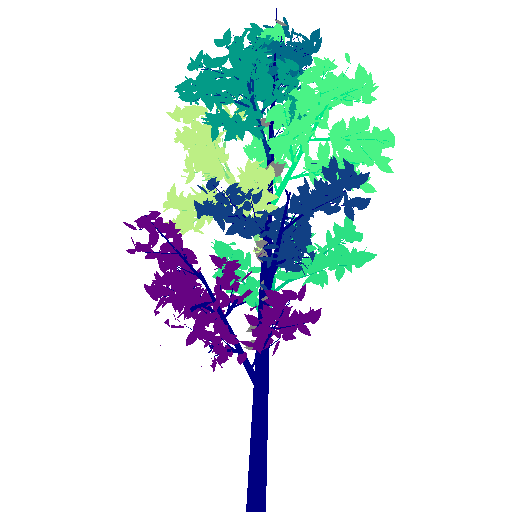
\includegraphics[width=0.30\textwidth]{./figures/dataPreExpanded.png}&

\includegraphics[width=0.30\textwidth]{./figures/dataExpanded.png}\\
(a)&(b)
\end{array}$
\end{center}
\caption[Ukázka expanze dat]%
{Ukázka expanze dat (změněna barevnost pro lepší zřetelnost). (a) před expanzí, (b) po expanzi.\label{fig:dataExpansionExample}
}
\end{figure}

Textury daného typu (barevné, normálové, \dots) jsou následně sloučeny dohromady (viz obr.~\ref{fig:joinTextures}). Děje se tak z důvodu ušetření texturovacích jednotek, jejichž počet je hardwarově omezen. Pro LOD1 s 3 směry řezů po 3 vrstvách a 4 sadami textur by tedy bylo nutné připojit $ (3 \times 3 \times 4 ) = 36 $ textur. Místo toho stačí připojit pouze 4 sloučené textury, což představuje značnou úsporu.
%%%
% obrazek pred a po expanzi dat
%
\begin{figure}[!hbt]
\begin{center}
\fbox{
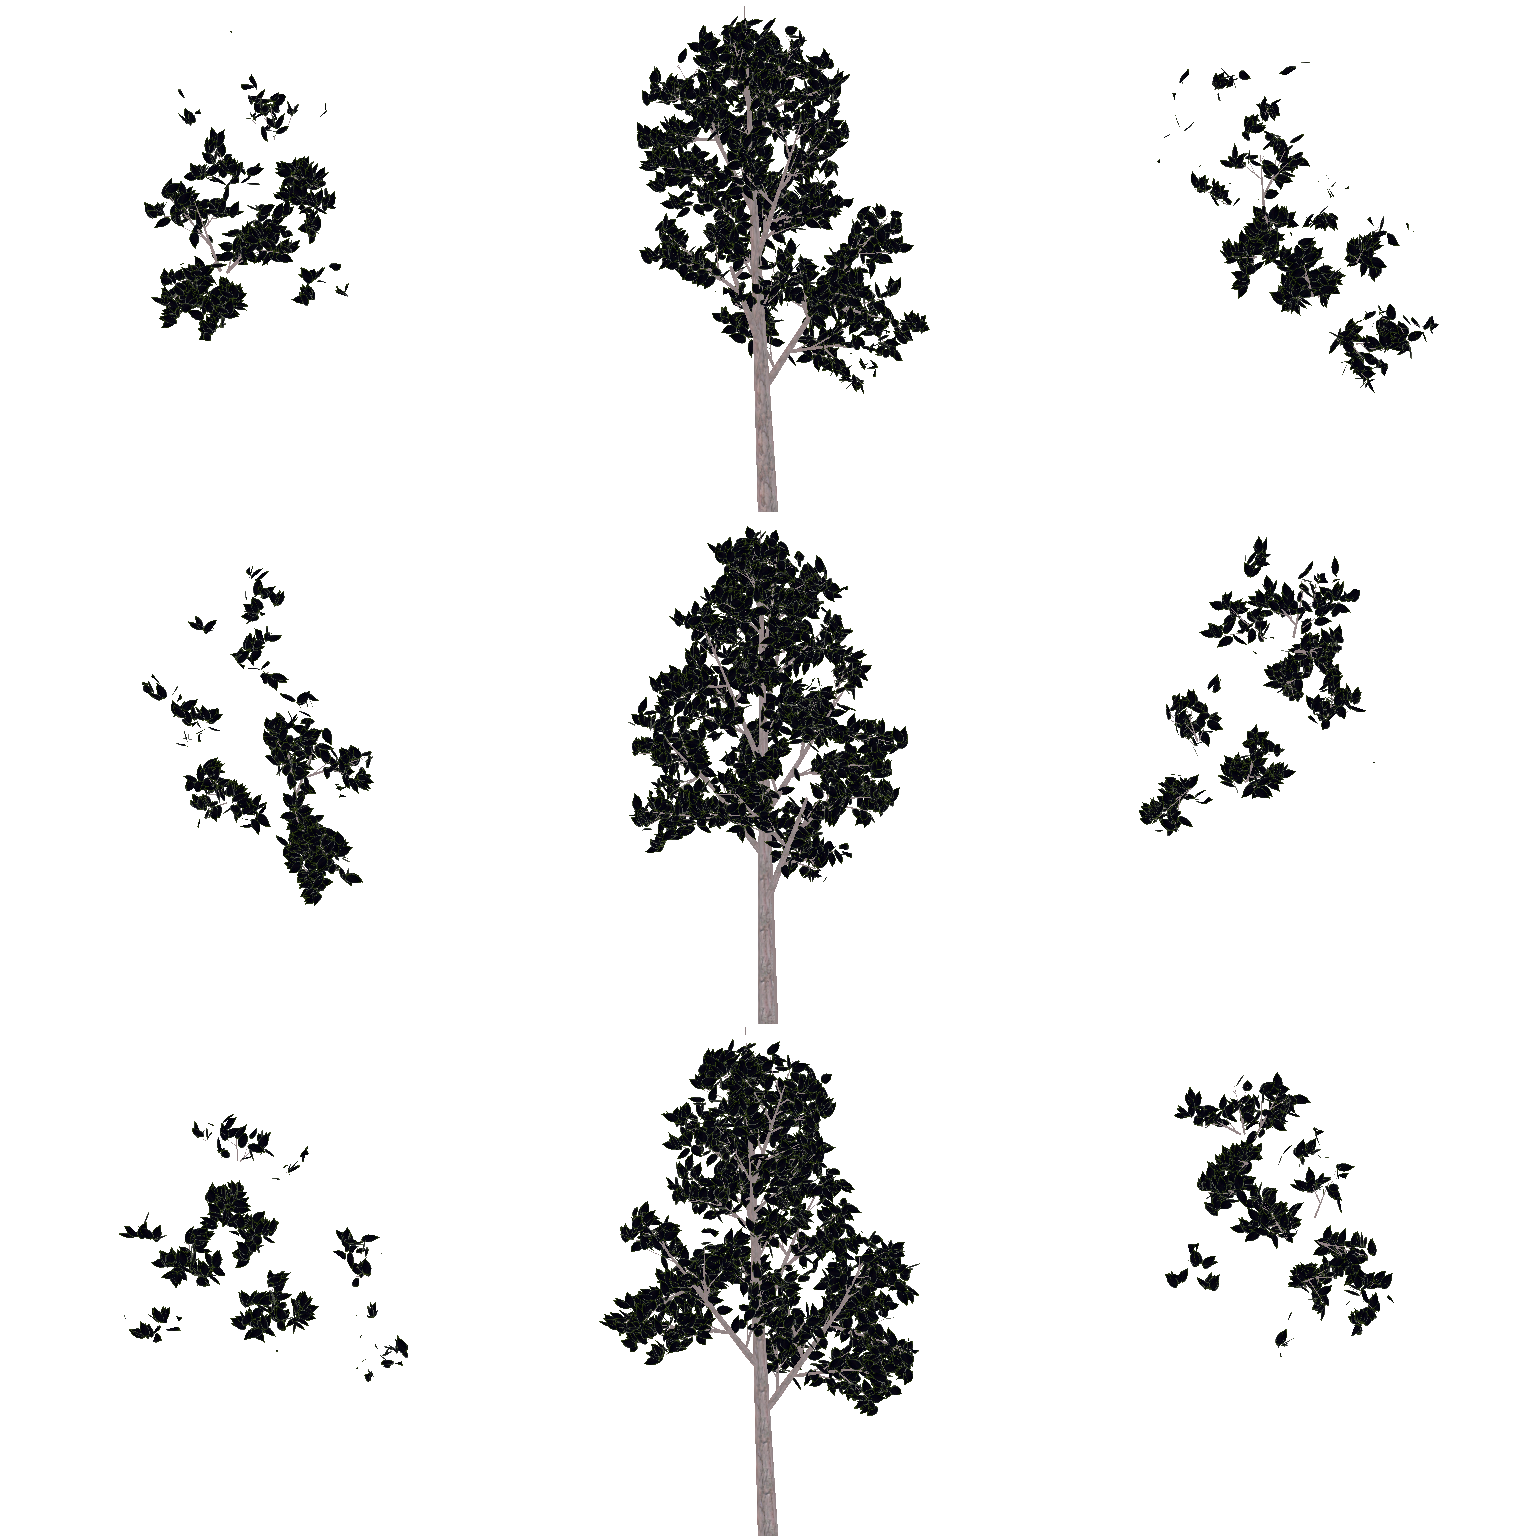
\includegraphics[width=0.4\textwidth]{./figures/joinTextures.png}
}
\end{center}
\caption[Slučování textur]%
{Slučování textur. Ukázka sloučení barevných textur pro LOD1 do jedné textury. .\label{fig:joinTextures}
}
\end{figure}

\pagebreak

Zásadní pro provádění animace v LOD operujícími nad trsy řezů je rovněž datová textura s informacemi o jednotlivých větvích. Tato textura obsahuje záznam pro každou větev, který obsahuje infromace o počátku větve v souřadném systému řezu, bázové vektory větve převedené rovněž do souřadného sytému řezu, projektovanou délku a pohybové vektory směru posunu v šumové textuře. Tyto informace se různí pro různé směry řezů a musí být tudíž zapsány i do textury pro každý směr zvlášť.


Data v datové textuře jsou tedy následující:
\begin{table}[!hbt]
\catcode`\-=12
\begin{center}
\begin{tabular}{c | c | c | c | c } 
 & \multicolumn{4}{c}{obsah textury}\\
 & \multicolumn{3}{c }{data řezu $j$} & data řezu $j+1$\\
$i+1$ & \multicolumn{3}{c |}{\vdots} & \vdots\\
\cline{1-5}
\multirow{4}{*}{$i$} 	& $\vec{o_s}.x$ 	& $\vec{r_s}.x$ 	&  $\vec{s_s}.x$ &  \multirow{4}{*}{\dots}\\
\cline{2-4}
				   	& $\vec{o_s}.y$ 	& $\vec{r_s}.y$  &  $\vec{s_s}.y$  & \\
\cline{2-4}
					& $\vec{mv}.x$ 	& $\vec{r_s}.z$  &  $\vec{s_s}.z$  & \\
\cline{2-4}
					& $\vec{mv}.y$  & $l_s$ 	&    & \\
\hline
$i-1$ & \multicolumn{3}{c |}{\vdots}&\vdots\\
\end{tabular}
\label{table:dataTexture}
\caption{Minimální sada dat uložená v datové textuře.}
\end{center}
\end{table}
\begin{figure}[!hbt]
\begin{center}

\includegraphics[width=0.05\textwidth]{./figures/branchDataTextureLOD1.png}
\end{center}
\caption[Ukázka části  datové textury pro LOD1]%
{Ukázka části datové textury pro LOD1. Číslo řádku $i$ odpovídá identifikátoru větve.\label{fig:branchDataTextureLOD1}
}
\end{figure}

%%%%%%%%%%%%%%%%%%%%%%%%%%%%%%%%%%%%%%%%%%%
\subsection{Dynamické parametry}
Aplikace nabízí možnost měnit dynamicky řadu parametrů souvisejících s animace stromů i s jejich zobrazováním. Nejpodstatnější jsou zejména tyto: \newline

\begin{tabular}{l} 
- směr větru\\
- síla větru\\
- amplituda větví (pro každou úroveň zvlášť)\\
- frekvence větví (pro každou úroveň zvlášť)\\
- amplituda listů\\
- frekvence listů\\
- prahy přechodů LOD\\
- sezóna\\
- směr světla\\
\end{tabular}

